\section{Static Electricity}

\begin{multicols}{2}


\section*{Concept of Static Electricity}


\subsection{Paper Jump}

\begin{center}
\includegraphics[width=0.3\textwidth]{./img/source/static-elec.png}
\end{center}

\begin{description*}
%\item[Subtopic:]{}
\item[Materials:]{Small pieces of paper, ruler, pen, balloon, salt and pepper (optional)}
%\item[Setup:]{}
\item[Procedure:]{Rub a pen, ruler or blown up balloon against your hair for about 30 seconds. Then bring it close to the small papers on a table.}
%\item[Hazards:]{}
%\item[Questions:]{}
\item[Observations:]{The small papers jump and cling to the object.}
\item[Theory:]{When you rub the object against your hair, electrons are transferred by friction to the object, giving it a negative charge. When the negatively charged object approaches the papers, the electrons in the papers are repelled downwards and the protons are attracted towards the top. When the object is close enough the positive charges on the tops of the papers jump and cling to the negatively charged object.}
%\item[Applications:]{}
\item[Notes:]{Try also with salt and pepper. The pepper jumps but the salt is too heavy and does not.}
\end{description*}

\vfill
\columnbreak

\subsection{Law of Electrostatics}

\begin{center}
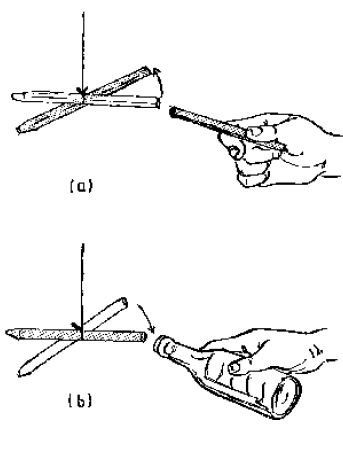
\includegraphics[width=0.4\textwidth]{./img/source/law-electrostatics.png}
\end{center}

\begin{description*}
%\item[Subtopic:]{}
\item[Materials:]{Plastic pens, wool cloth, sting, glass bottle, silk cloth (inside of a suit)}
%\item[Setup:]{}
\item[Procedure:]{Rub a plastic pen on your hair and bring it near a suspended pen charged in the same way. Repeat by bringing a glass bottle charged with silk or polyester near the suspended charged pen.}
%\item[Hazards:]{}
%\item[Questions:]{}
\item[Observations:]{The two charged pens repel each other, but the glass bottle attracts the charged pen.}
\item[Theory:]{\emph{Like charges repel and unlike charges attract}. The two pens are negatively charged after gaining electrons from the hair. The glass bottle is positively charged after giving up electrons to the silk.}
%\item[Applications:]{}
%\item[Notes:]{}
\end{description*}

\vfill
\columnbreak

\subsection{Electrostatic Induction}

\begin{center}
\includegraphics[width=0.4\textwidth]{./img/source/elec-induction.png}
\end{center}

\begin{description*}
%\item[Subtopic:]{}
\item[Materials:]{Ruler, aluminum foil, string}
%\item[Setup:]{}
\item[Procedure:]{Crumple a piece of foil into a ball and suspend it from a string. Charge a ruler by rubbing on your hair and bring it close to the foil ball without touching it.}
%\item[Hazards:]{}
%\item[Questions:]{}
\item[Observations:]{The aluminum ball is attracted by the charged plastic ruler.}
\item[Theory:]{The negatively charged ruler repels the electrons in the foil ball and attracts the protons, creating an induced \emph{dipole} in the ball. This is called \emph{electrostatic induction}.}
%\item[Applications:]{}
\item[Notes:]{Try different materials such as rubbing plastic on nylon, glass on silk, or latex on fur.}
\end{description*}

\subsection{Water Pull}

\begin{center}
\includegraphics[width=0.4\textwidth]{./img/source/comb-water-2.jpg}
\end{center}

\begin{description*}
%\item[Subtopic:]{}
\item[Materials:]{Comb, water stream or tap}
%\item[Setup:]{}
\item[Procedure:]{Rub a comb in your hair for about a minute. Then bring the comb close to a narrow stream of water from a tap or bottle.}
%\item[Hazards:]{}
%\item[Questions:]{}
\item[Observations:]{The water is pulled towards the comb.}
\item[Theory:]{The comb gains electrons from the hair and becomes negatively charged. The protons in the water molecules are attracted to the electrons in the comb. The water is said to have an \emph{induced dipole}.}
%\item[Applications:]{}
%\item[Notes:]{}
\end{description*}

\subsection{Charged Balloon}

\begin{center}
\includegraphics[width=0.25\textwidth]{./img/source/charged-balloon.jpg}
\end{center}

\begin{description*}
%\item[Subtopic:]{}
%\item[Materials:]{Balloon}
%\item[Setup:]{}
\item[Procedure:]{Rub a balloon on a wool cloth or hair and then place it against the ceiling.}
%\item[Hazards:]{}
%\item[Questions:]{}
\item[Observations:]{The charged air balloon sticks to the ceiling.}
\item[Theory:]{The negative charge on the balloon repels some of the electrons in
the ceiling away from the surface. This leaves the surface positively charged and so the
negative balloon is attracted by the ceiling.}
%\item[Applications:]{}
\item[Notes:]{The experiment should be carried out during dry weather.}
%Otherwise moisture in the air will
%neutralize the charges and the balloon will not stick to the ceiling.}
\end{description*}

%==================================================================================================%

\section*{Electroscope}


\subsection{Simple Electroscope}

\begin{center}
\includegraphics[width=0.4\textwidth]{./img/source/simple-electroscope.jpg}
\end{center}

\begin{description*}
%\item[Subtopic:]{}
\item[Materials:]{Plastic strips, duster, plastic spoon}
\item[Setup:]{Cut two strips of plastic and fix to a piece of wood. Charge the strips by rubbing with a clean duster.}
\item[Procedure:]{Bring a charged plastic spoon between the charged strips and then your finger.}
%\item[Hazards:]{}
%\item[Questions:]{}
\item[Observations:]{The charged strips are repelled further by the charged spoon, but attracted to the finger.}
\item[Theory:]{The finger attracts the strips because the body is earthed, so it becomes positively
charged relative to the two negatively charged strips.}
%\item[Applications:]{}
%\item[Notes:]{}
\end{description*}

\columnbreak

\subsection[Construction of a Simple Electroscope]{Construction of a Simple \hfill \\ Electroscope}

\begin{center}
\includegraphics[width=0.25\textwidth]{./img/al-leaf-electroscope.png}
\end{center}

\begin{description*}
%\item[Subtopic:]{}
\item[Materials:]{Clear jar with a plastic cap, iron nail, small piece of aluminium foil, glue, ruler or glass and silk}
\item[Setup:]{Insert the nail into the cap so that about 1 cm remains above the top. Use glue to secure it in place. Cut a piece of aluminium foil 0.5~cm by 2~cm. Glue one end of the foil (only the tip) to the nail about 2~cm from the bottom. Bend the foil so it can swing easily. Close the cap with the nail and foil.}
\item[Procedure:]{Bring a charged object near the nail and notice any deflection in the leaf.}
%\item[Hazards:]{}
%\item[Questions:]{}
\item[Observations:]{The leaf deflects from the nail.}
\item[Theory:]{The charged object repels the opposite type of charge in the nail, which moves down the nail and into the leaf. The like charges on the nail and leaf repel each other, causing a deflection to occur.}
%\item[Applications:]{}
%\item[Notes:]{}
\end{description*}

%\vfill
%\columnbreak

%\subsection{Detection of Charges}
%
%\begin{center}
%\includegraphics[width=0.4\textwidth]{./img/source/.png}
%\end{center}
%
%\begin{description*}
%%\item[Subtopic:]{}
%\item[Materials:]{Electroscope (see above activity), pen, glass, silk}
%%\item[Setup:]{}
%\item[Procedure:]{}
%\item[Hazards:]{}
%\item[Questions:]{}
%\item[Observations:]{}
%\item[Theory:]{}
%\item[Applications:]{}
%\item[Notes:]{}
%\end{description*}

\subsection{Simple Detector}

\begin{center}
\includegraphics[width=0.45\textwidth]{./img/vso/simple-detector.jpg}
\end{center}

\begin{description*}
%\item[Subtopic:]{}
\item[Materials:]{Paper, needle/pin, sand-filled can, ruler}
\item[Setup:]{Mount a strip of paper 10 cm by 2 cm on a needle supported by a sand-filled can.}
\item[Procedure:]{Bring a charged object (ruler or pen rubbed on hair or glass rubbed with silk) close to the paper.}
%\item[Hazards:]{}
\item[Questions:]{Which way does the paper move for different charged objects?}
%\item[Observations:]{}
\item[Theory:]{The paper will deflect when a charged object is brought near due to induction. Any charge on the paper can be detected based on whether it is attracted to the object (same charge) or repelled (opposite charge).}
%\item[Applications:]{}
%\item[Notes:]{}
\end{description*}

\columnbreak

%==================================================================================================%

\section*{Capacitors}

\subsection{Paper Capacitor}

%\begin{center}
%\includegraphics[width=0.4\textwidth]{./img/source/.png}
%\end{center}

\begin{description*}
%\item[Subtopic:]{}
\item[Materials:]{Aluminum foil, paper, dry cell, voltmeter, wires, tape}
\item[Setup:]{Cut 2 sheets of aluminum foil (e.g. 20 cm $\times$ 20 cm).}
\item[Procedure:]{Place several sheets of paper between the foil sheets. Connect each foil sheet to a terminal of the dry cell using tape. Connect a voltmeter across the foil sheets.}
%\item[Hazards:]{}
%\item[Questions:]{}
\item[Observations:]{The foil sheets become charged by the battery and show a small potential difference on the voltmeter.}
\item[Theory:]{\emph{Capacitors} are devices that store charge between two conducting plates. Placed between the plates is an insulating material known as a \emph{dielectric}. The capacitance of a capacitor depends on the surface area of the conducting plates, the distance between them, and the dielectric material.}
%\item[Applications:]{}
%\item[Notes:]{}
\end{description*}


\end{multicols}

\pagebreak